\section{Problem No.2} \label{sec:prob2}
\subsection{Problem Description:} 
Write programs to solve 
$$
u_{t} = \Delta u \;\; on \;\; \Omega = (0,1) \times (0,1)\\
u=0 \;\; on \;\; \partial \Omega \\
u(x,y,0) = exp(-100((x-0.3)^{2} + (y-0.4)^{2}))
$$
to time t=1 using forward Euler and \cn. For \protect{\cn} use a fixed time step of $\Delta t =0.01$, and for forward Euler use a time step just below the stability limit. For \protect{\cn} use Gaussian elimination to solve the linear system that arises, but make sure to account the banded structure of the matrix.
\begin{enumerate}
\item Time your codes for different grid and compare the time to solve using forward Euler and \cn. 
\item In theory, how should the time scale as the grid is refined for each algorithm? How did the time scale with the gird size in practice?
\item For this problem we could use and FFT-based Poisson solver which will perform the direct solve in $\mathcal{O}(Nlog(N))$, where $N$ is the total number of grid points. We could also use multigrid and perform the solve in $\mathcal{O}(N)$ time. How should the time scale as the grid is refined for \protect{\cn} if we used an $\mathcal{O}(N)$ solver? 
\end{enumerate}

\subsection{Solution:}
\paragraph{Part 1:} We record the timing for different grid resolution for both forward Euler and \protect{\cn} schemes and the timings are show in Figure \ref{fig:time}. 


\begin{figure}[tbh]
 \centering  
  \begin{tabular}{c|c|c}
\begin{tabular}{ |p{2cm}|p{2cm}|p{2cm}|p{2cm}|p{2cm}|p{2cm}}
 \hline
 \multicolumn{3}{|c|}{Forward Euler} &  \multicolumn{3}{c}{\protect{\cn}}\\
 \hline
 $\Delta t$ &  $\Delta x$  & time & $\Delta t$ &  $\Delta x$  & time\\
 \hline
 0.000976 & 0.0625  & 2.0E-06   &  0.01  & 0.0625  & 1.00E-06\\
 0.000244 & 0.03125 & 2.0E-07   &  0.01  & 0.03125 & 1.00E-05\\
 6.1E-05  &  0.01563 & 8.0E-05  &  0.01  & 0.01563 & 0.000108\\
 1.53E-05 & 0.00782 & 0.001047  &  0.01  & 0.00782 & 0.000831\\
 3.81E-06 & 0.00391 & 0.015268  &  0.01  & 0.00391 & 0.011299\\
 \hline
\end{tabular} 
   \end{tabular}   
        
   {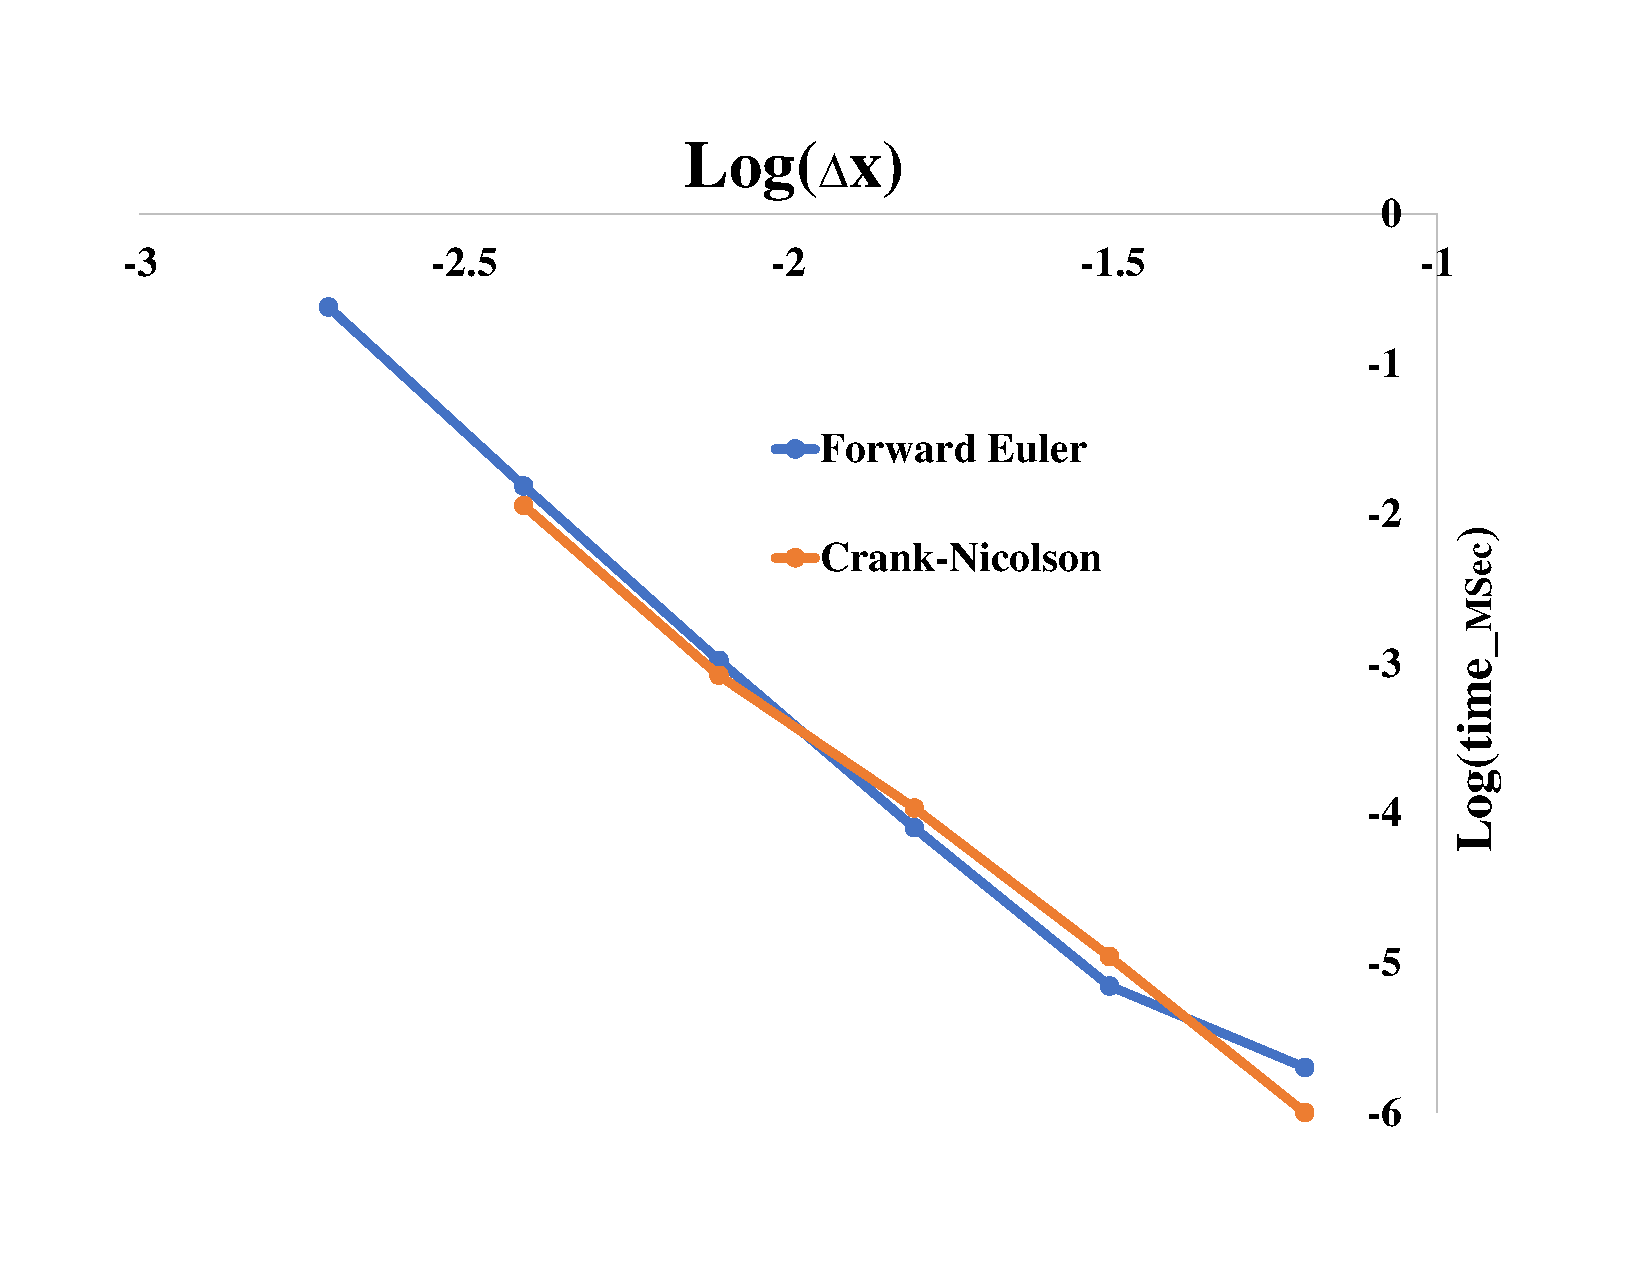
\includegraphics[width=0.6\linewidth]{fig/timing.pdf}}
  \caption{Timing of the refinement study on forward Euler and \protect{\cn} schemes applied on problem 2. The tables show the actual time in milliseconds and the figure shows the curve drawn on a log-log scale to indicate the order of the complexity.}
   \label{fig:time}
\end{figure} 


   
\paragraph{Part 2:} With \protect{\cn}, the system of equations is banded matrix which can be solved using LU-decomposition \cite{press1987numerical} which has complexity of $\mathcal{O}(N^2)$ for $N$ unknowns. For this problem, the number of unknowns at each time step is $N_{x}-2 \times N_{y}-2$, where $N_{x}$ and $N_{y}$ is the number of grid points in x and y direction respectively. Thus, it is expected for the banded matrix solver (and thus for \protect{\cn} scheme) to be of order $\mathcal{O}(N^2)$. For the explicit forward Euler scheme, the number of operations is of order of the number of unknowns. Thus, the complexity is of order $\mathcal{O}(N^2)$ for forward Euler. 

There is hidden overhead with forward Euler due to its stability criterion as we have to perform temporal refinement as we do spatial refinement. In contrast to \protect{\cn} which is unconditionally stable. For forward Euler, the method is only stable only when $\frac{\Delta t}{\Delta x^{2}} \leq \frac{1}{4}$. Since we take time steps just below the stability limit, the complexity of forward Euler at each time step increases to be $\mathcal{O}(N^{4})$. Thus if we double the space steps ($N_{x}$ and $N_{y}$) we should exhibit 16 times increase in time. For \protect{\cn}, doubling the space steps would give the same increase in time. 

The slope of the curve in Figure \ref{fig:time} is 3.4 for both schemes which deviates by a factor of $15\%$ from the what is expected. For \protect{\cn}, this could be justified since we don't go through the LU-decomposition of the banded matrix at every solution step. Instead, half the work done once (finding the pivot), and the other half of the work is solved per time step (backward and forward substitution). For forward Euler, it is not clear why such deviation occurs. 


\paragraph{Part 4:} Using a $\mathcal{O}(N)$ solver, the time scale will be four for \protect{\cn} since no temporal refinement is needed given the same reasoning we give for a $\mathcal{O}(N^{2})$ solver.